%% Comment out the first line during final production.

\renewcommand{\thechapter}{2}
\chapter{Study Regions}
\label{chap:study regions}

\begin{linenumbers}[1]

\section{Overview of the Lower Arkansas River Valley in Colorado}
\label{overview of the lower arkansas river valley in colorado}

The Upstream Study Reach (USR) extends from just west of Manzanola to near Las Animas and is representative of the hydrology, soil, crop, and irrigation conditions upstream of John Martin Reservoir.  The Downstream Study Reach (DSR) is representative of the conditions downstream of John Martin Reservoir.  It extends from Lamar to the Colorado-Kansas state line.  Both study reaches are located in the LARV which starts at the outlet of Pueblo Reservoir, approximately \SI{10.5}{\kilo\meter} (\SI{6.5}{\mile}) miles west of Pueblo, Colorado and extends into Kansas.  This study is only concerned with the portions of the Arkansas River and LARV in Colorado.  All portions of the LARV in Colorado are within Division 2 of the Colorado Department of Water Resources (CDWR).  Division 2 offices are located in Pueblo, Colorado.  The CDWR is the state agency responsible for the legal administration of all surface and sub-surface waters in the State of Colorado.  Figure \ref{map:LARV map} shows the location of the LARV, USR, DSR, and adjacent irrigated valley lands that contribute to the non-point source (NPS) return flows and loads to the study reaches in this thesis.

\afterpage{%
	\clearpage%
	\begin{landscape}
	\begin{figure}
		\centering
			\includegraphics[width=9in]{"Figures/Map/LARV"}
			\caption[Lower Arkansas River Valley.]{Lower Arkansas River Valley.}
			\label{map:LARV map}
	\end{figure}
	\end{landscape}
}

% Regional Geology
\subsection*{Regional Geology of the LARV.}
The LARV is wide, with widths up to approximately \SI{20}{\kilo\meter} (\SI{12.5}{\mile}), but shallow with maximum elevation differences approaching \SI{130}{\meter} (\SI{425}{\foot}).  The un-confined aquifer sits in alluvium made of a series of late Cambrian to Tertiary sedimentary formations \parencite{darton1906}.  The bedrock underlying the alluvium consists primarily of marine-derived shales of the Pierre, Niobrara, Carlisle, and Graneros series and limestones for most of the valley.  As the river nears the Colorado-Kansas border, the bedrock is Dakota sandstone \parencite{moore1967} .  The river is characterized as a shifting sand channel that meanders along the alluvial flood plain which is incised into the flood way.  The alluvial aquifer and the Arkansas River and its tributaries have a strong hydraulic connection with the Arkansas River \parencite{konikow1974}.

Evidence indicates that the marine-derive shale bedrocks that underly most of the LARV and their weathered residuum yield a variety of salts, Se, and U under the dissolving action of natural and irrigation flows \parencite{zielinski1995,zielinski1997,gates2009,Bailey2012}.  In the US, selenium is readily abundant in some, but not all areas west of the western Dakotas, Nebraska, Kansas, and Oklahoma to the west cost \parencite{Painter1940}.  Figure \ref{fig:USSeMap} is a set of geochemical distribution maps developed by the U.S.G.S. Mineral Resourses Program that shows the distribution of Se in the conterminous U.S. in the \SIrange{0}{5}{\centi\meter} layer, the top soil (A horizon) layer, and the parent rock (C horizon) layer \parencite{2014Smith}.

\afterpage{%
	\clearpage
	\begin{figure}
		\centering
		\includegraphics[scale=.9]{"Figures/Map/USSeMap"}
		\caption[Distribution of Se in Soil in the Conterminous United States.]{Distribution of Se in Soil in the Conterminous United States \parencite{2014Smith}.  This is a composite of three individual maps.}
		\label{fig:USSeMap}
	\end{figure}
}

\subsection*{Regional Climate and Hydrology of the LARV}

Regionally, the climate is arid with large temperature fluctuations.  Most of the rainfall comes during the growing season in the form of heavy thunderstorms.  Summers are hot with an average high temperature of \ang{93}F (\ang{34}C) and winters are cold, with an average low temperature of \ang{14}C \ang{-10}C.  Snowfall is usually light, but is prone to drifting with the low humidity and moderately high velocity, steady winter winds.

The historic stream flows show considerable seasonable variability.  Most of the total annual flow is influenced primarily by snow melt and runoff in the Upper Arkansas River Basin, above Pueblo Reservoir.  Additionally, groundwater base flow, runoff from precipitation events in the Eastern Colorado plains, and releases from Pueblo and John Martin Reservoirs in compliance with operational rules contribute to flow rates \parencite{Miller2010}.

Average annual precipitation within the LARV ranges between \SI{31.52}{\centi\meter} (\SI{12.41}{\inch}) in Pueblo, and varies eastwardly to \SI{39.65}{\centi\meter} (\SI{15.61}{\inch}) in Holly.  Figure \ref{map:LARVRainfall} is a map of the LARV with the Average Annual Precipitation from 1981 - 2010 as reported by the U.S.D.A N.R.C.S.  Average reference ET ($ ET_{Ref} $) during the irrigation season (15 March - 15 November) is \SI{1.3}{\meter} (\SI{4.25}{\foot}) based on data collected from CoAgMet weather stations over the period 1992 - 2008 \parencite{clifford2009}.  The Arkansas River riparian zone in the flood way is primarily characterized by heavy growth of Russian Olive (\textit{Elaeagnus angustifolia}), multiple species of salt cedar (\textit{Tamarix}), willows and other non-native species that are major contributors to regional evapo-transpiration (ET) losses \parencite{Nagler2010a}.

\afterpage{%
	\clearpage%
	\begin{landscape}
		\begin{figure}
			\centering
			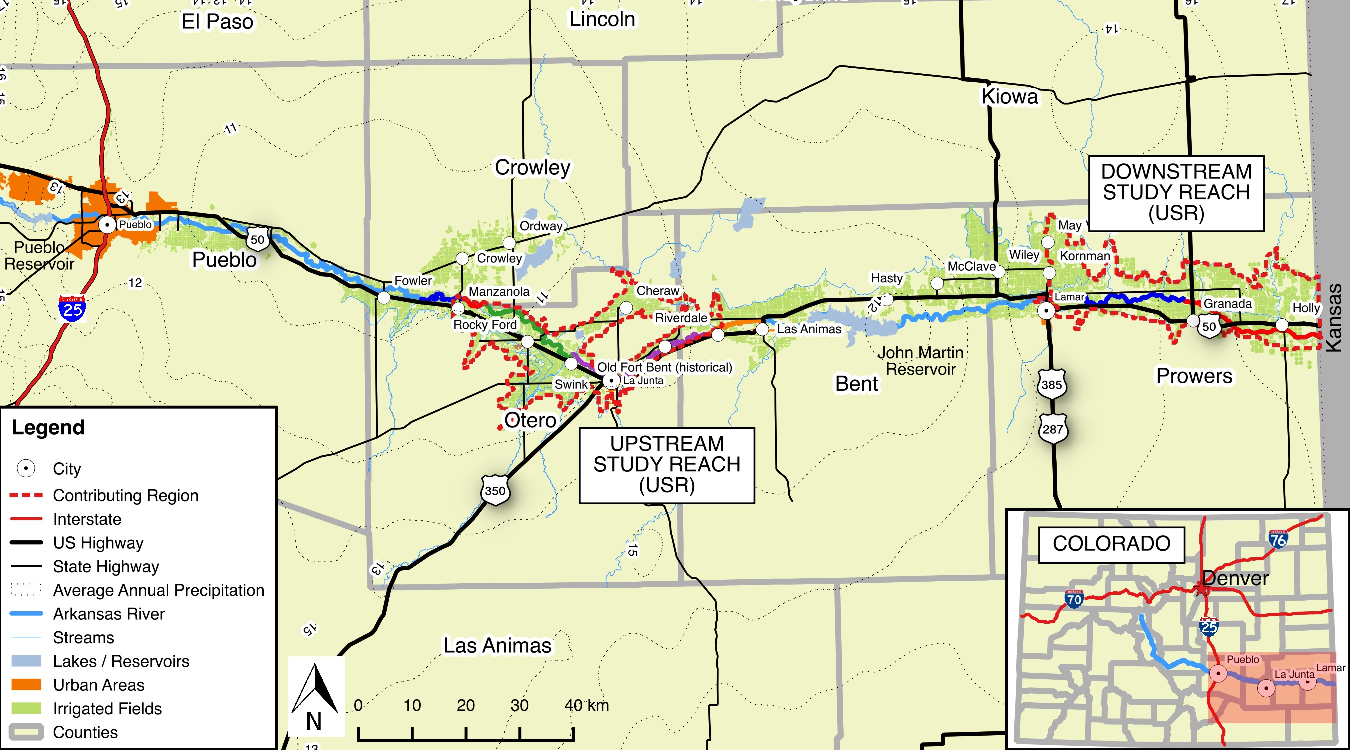
\includegraphics[width=9in]{Figures/Map/LARVRainfall}
			\caption[Precipitation in the LARV]{Precipitation in the LARV.  Values on the isolines are reported as inches of average annual rainfall.}
			\label{map:LARVRainfall}
		\end{figure}
	\end{landscape}
}

\subsection*{Anthropogenic Factors for the LARB Study Regions.}

Historically, prior to the advent of irrigated agriculture in the Ark River Basin during the 19th century, groundwater recharge in the basin occurred primarily from infiltration of precipitation through the unsaturated zone and from infiltration of surface water from losing streams.  By mid-1880s, the waters of the Arkansas R. and its tributaries were fully appropriated for normal or average years \parencite{Abbott1985}.  In areas where surface water was diverted for irrigation, infiltration of irrigation water from canals and fields became a primary source of groundwater recharge.  Natural recharge is about 0.08 inches/year in the southeast corner of the state \parencite{Wolock2003}.

The LARV river-aquifer system supplies water to towns and industries through shallow aquifer wells.  Water is returned either directly to the river after treatment or into the aquifer through groundwater seepage from treatment lagoons.  Water supplied to these entites is a very small portion when compared to the demand from agriculture in the valley.

Agriculture is the primary industry in the LARV with approx 270,00 acres irrigated \parencite{Bailey2015,Miller2010}.  There are 25 main irrigation canals in the LARV with diversion structures crossing the river.  Many fields near the river drain excess irrigation water directly back to the river \parencite{Bailey2012,Morway2013}.  There are also about 2,400 groundwater pumping wells that tap into the riparian aquifer, thereby taking water, albeit indirectly, from the river.  The floodplain is characterized by heavy agriculture on fertile soils.  The region is known for a wide variety of crops including but not limited to alfalfa, corn, grass hay, wheat, sorghum, dry beans, cantaloupe, watermelon, and onions in order of cropped area (USDA NASS Colorado Field Office 2009).  There are also a few diaries and cattle feed lots.  Most fields are irrigated using surface-irrigation methods with less than about 5\% irrigated with sprinklers or drip lines.  Surface and sprinkler irrigation efficiencies are varied depending on the crop and location \parencite{Bailey2012Phd} ref{Gates et al 2015}

Precipitation in the LARV is substantially insufficient to support crop production by about \SI{0.9}{\meter} (\SI{3}{\foot}).  It has been estimated that appropriated water rights in the LARV exceede the annual native river flow by as much as 40\% in a low flow year \parencite{cain1985,sutherland1988}.  Additional water is provided by releases from Pueblo and John Martin Reservoirs which store water during the winter period.  Some of this water is provided through trans-basin transfers through the Fryingpan-Arkansas Project.

Seepage from canals contributes significantly to the water quantity and quality in LARV aquifer.  Canals are constructed at higher elevations, promoting the surface transport of water over long distances to fields.  This elevation difference also places a higher hydraulic gradient between the canal and aquifer.  Canals, as a rule, are not constructed such that groundwater infiltrates into the canal channel.  The entire process promotes the movement of water and dissolved constituents, including \nitrate, Se, U, and salts directly into the aquifer.  Additionally, a significantly large quantity of the total canal length in the LARV is located away from the river.  This has two results.  Since the aquifer is receiveing recharge water from the canals, it acts as a reservoir, delaying the return of that water to the river channel.  This result is seen during low flow conditions when the river channel still contains water, even though historic conditions would tell us otherwise.  The second result is that dissolved constituents are introduced into the aquifer where it is the shallowest, along the edges of the valley.  This brings \nitrate and dissolved oxygen into contact with the Se bearing bedrock before either can be siginficantly depleted through other redox reactions \parencite{Bailey2012Phd,Morway2013}.

%\todo{--  Paragraph describing how irrigation and flows from canal seepage induce high concentrations of salt, Se, U, and nutrients throug evapo-transpiration and dissolution processes.  Tell how do these solutes travel to the stream system driven by the large groundwater gradients .}

%\todo{-- Briefly describe the distinctions between the geologic sources of Se (Ref: Gates et al 2009) and irrigation practices in the regions feeding the USR and DSR (Ref: Gates et al 2012, 2015) that would influence return flows and Se loading along these reaches. --}


\clearpage{}
\section{Upstream Study Reach and Surrounding Region}
\label{sec:upstream study region and river reach}
The upstream boundary of the USR starts immediately downstream of the Catlin Canal diversion dam.  The dam is approximately 4.5 miles (mi) (7 km) west of the intersection of U.S. Highway 50 and State Highway 207 in Manzanola and 4.5 mi (7 km) east of the intersection of U.S. Highway 50 and State Highway 164 in Fowler.  The USR extends along approximately 61.5 mi (99 km) of the river to where U.S. Highway 50 crosses the Arkansas River north of Las Animas.  All portions of the USR are in CDWR Division 2, Water District 17 which extends from Fowler to Las Animas.  There are three main tributaries, multiple minor tributaries, five main irrigation canals, and one return canal (for augmentation flow) are present in the USR.  Figure \ref{fig:USR map} shows the extent and approximate path of the USR and the irrigated region supplyiing return flow to the reach.

\afterpage{%
	\clearpage%
	\begin{landscape}
	\begin{figure}
		\centering
		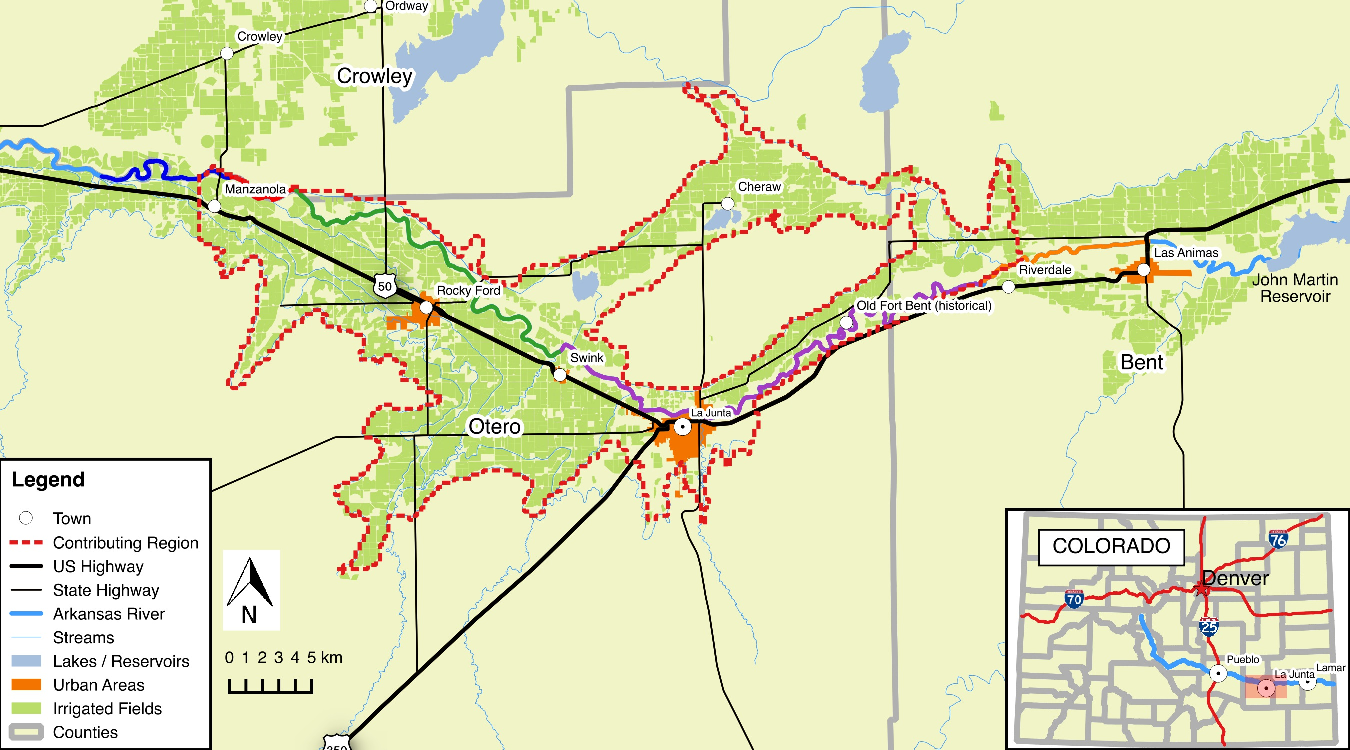
\includegraphics[width=9in]{Figures/Map/USR}
		\caption[Upstream Study Reach.]{Upstream Study Reach.  River segments within the USR are color coded.}
		\label{fig:USR map}
	\end{figure}
	\end{landscape}
}

The USR is separated into five segments given designations from "A" to "E" (Figure \ref{fig:USR map}).  Segments are geographically separated by irrigation canal diversion dams.  Segment B is the only segment that does not contain a stream gauge on the main stem of the river.  It is relatively short and has an additional diversion dam within its boundary.  Typically, significantly different flows pass through the main channel of the river within each segment.  Segments were defined to provide boundaries for river storage volume calculations.  Within each segment, except for segment B, the water surface level is determined primarily by flowrate, hydraulic geometry, and hydraulic resistance.  Knowledge of the water surface level is necessary for estimating the river storage volume.  A discussion of the river geometry analysis and storage volume calculation is provided in sections \ref{sec:River Survey} and \ref{sec:River Volume Change}. 

Figure \ref{fig:USR line map} is a line diagram representing the major flow paths in the USR.  This diagram is not to scale and depicts only the major canals and tributaries.  The segments within the reach are color coded.  Four canal diversion dams separate the segments.  Points in Figure \ref{fig:USR line map} designated as "Water Quality" are locations where CSU field technicians routinely took water samples for analysis.  A discussion of the sampling and analysis methods is presented in section \ref{sec:field data collection}.

\afterpage{%
	\clearpage%
	\begin{landscape}
	\begin{figure}
	\centering
		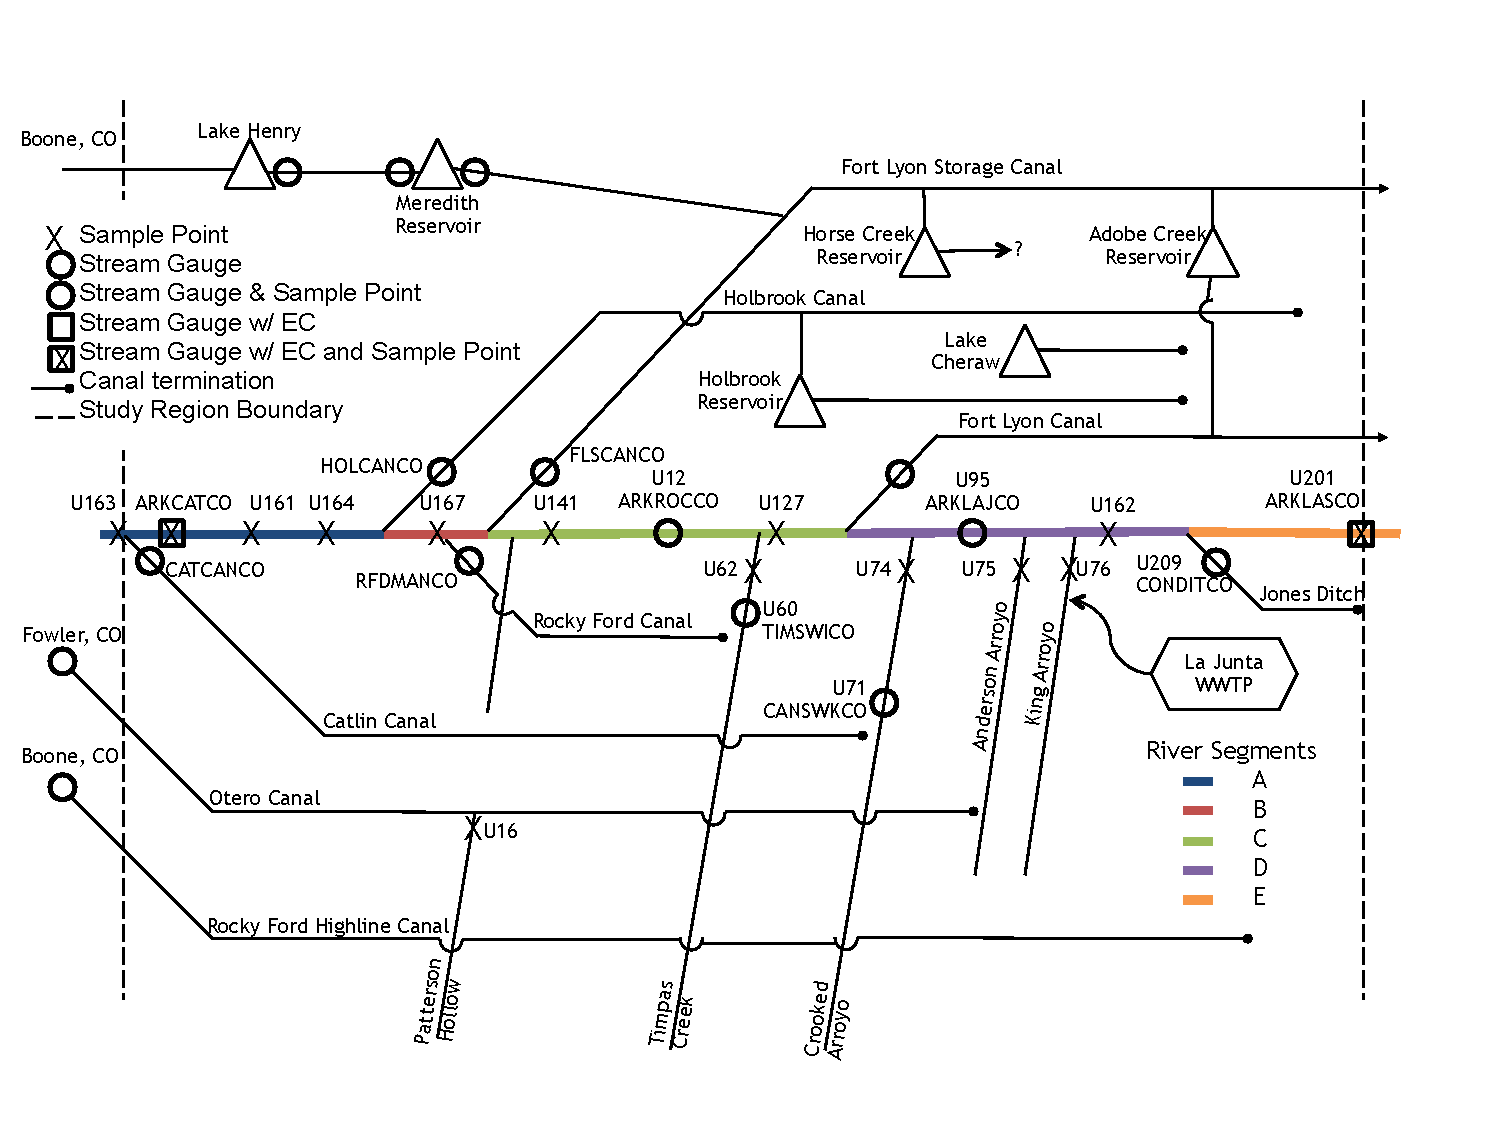
\includegraphics[width=9in]{Figures/LineDiagram/USRLineDiagram}
		\caption[Upstream Study Reach Flow Diagram.]{Upstream Study Reach Flow Diagram.}
		\label{fig:USR line map}
	\end{figure}
	\end{landscape}
}

The main tributaries are perennial and supply water to the Arkansas River under most conditions.  These tributaries are Timpas Creek, Crooked Arroyo, and Horse Creek.  Most of the minor tributaries are usually dry and only convey water during larger rainfall events and flood conditions.  All three major tributaries have a significant portion of their flows provided by agricultural runoff.

There are two minor tributaries that provide low volume, perennial flows to the Arkansas River: King Arroyo and Anderson Arroyo.  King Arroyo is assumed to be primarily fed by La Junta Waste Water Treatment Plant (WWTP) effluent.  The La Junta Water Treatment Plant (WTP) effluent spills into Anderson Arroyo.  It is currently unknown what groundwater and other flows contribute to the discharge from King or Anderson Arroyos.  No discharge data are provided for the La Junta WTP due to the very low discharge rates.  The discharge from the La Junta WWTP is included in the models.  

Patterson Hollow, a poorly-defined natural drainage, is depicted on the line graph as connected to the Arkansas River.  Flows from the upper reach of Patterson Hollow are diverted to the Otero Canal.  The reasons for the diversion are unknown, but it is speculated that the majority of the flows upstream of Otero Canal are irrigation returns and the diversion was an attempt to re-use valuable irrigation water.  Regardless, since Patterson Hollow, for the most part, was separated from the Arkansas River, it was not included in this study.

The five major canals diverting water from the Arkansas River along the USR are Holbrook Canal, Rocky Ford Canal, Fort Lyon Storage Canal, Fort Lyon Canal, and Jones Ditch.
The Rocky Ford Return Canal is the only monitored canal returning augmentation water to the Arkansas River in the USR.  
The Rocky Ford Return Canal diverts water from the Rocky Ford Canal and returns it directly to the Arkansas River. 
This system is in place to monitor and augment flows in conjunction with trans-basin flows used by the City of Aurora.  
The Otero and Rocky Ford Highline Canals run parallel to the USR.  They divert water from the Arkansas River upstream of the USR upstream boundary.  
Overflows from these two canals pass through the tributary gauge in Crooked Arroyo.

\clearpage{}
\section{Downstream Study Reach and Surrounding Region}
\label{sec:downstream study region and river reach}

The DSR begins at the U.S. Highway 50/U.S. Highway 287 Arkansas River crossing in Lamar, Colorado, and extends approximately 71 km to the Colorado/Kansas state line (Figure \ref{fig:DSR map}).  Figure \ref{fig:DSR line map} is a line diagram representing the flow structure within the DSR.  Similar symbology is used on these maps as in Figures \ref{fig:USR map} and \ref{fig:USR line map} for the USR.  For a period of time, there were four tributaries and drains in the DSR where flows were measured mannually gauged on an infrequent basis.  The results of the this stream gauging activity do not affect the calculation or analysis of this study, but will be discussed in the conclusion.  The entirety of the DSR lies within CDWR Division 2, District 67 and contains two major tributaries, multiple minor tributaries, and one irrigation canal. 

\afterpage{%
	\clearpage%	
	\begin{landscape}
	\begin{figure}%[htbp]
		\centering
		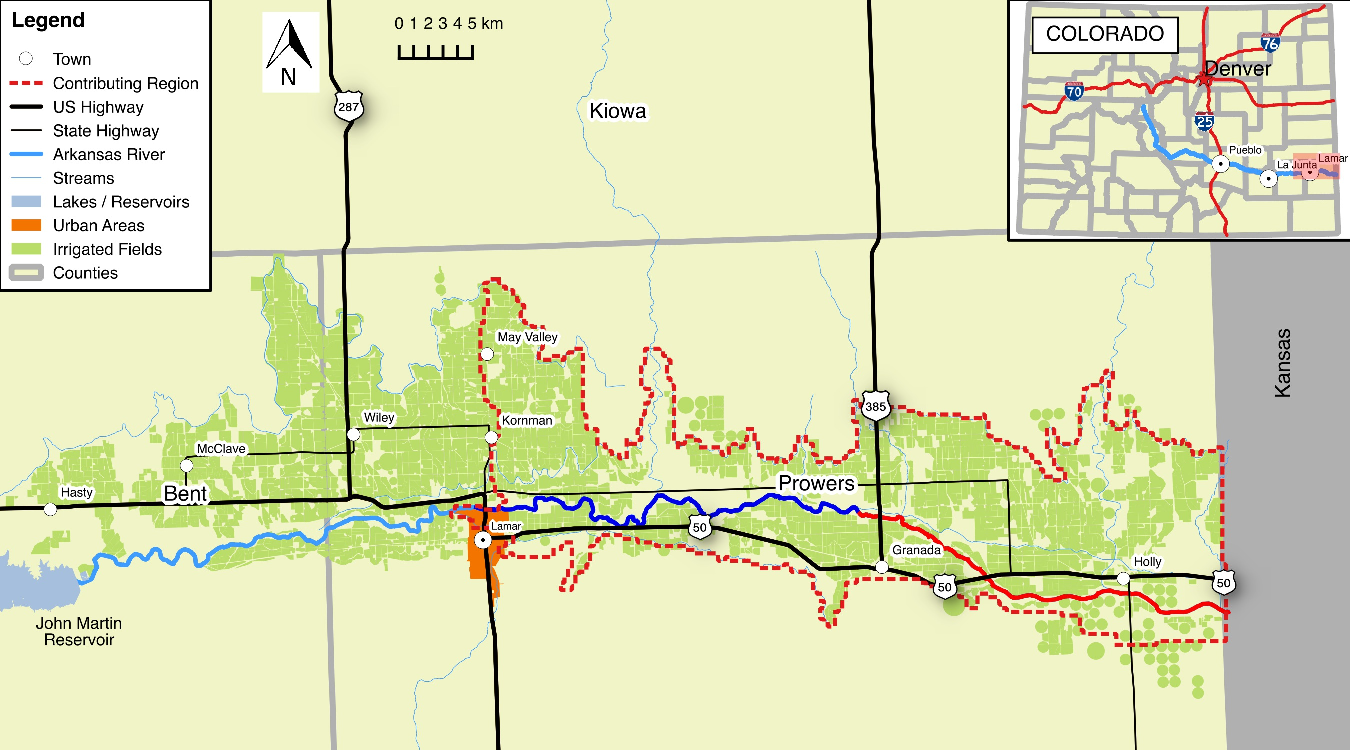
\includegraphics[width=9in]{Figures/Map/DSR}
		\caption[Downstream Study Reach.]{Downstream Study Reach.  River segments within the DSR are color coded.}
		\label{fig:DSR map}
	\end{figure}
	\end{landscape}
}

\afterpage{%
	\clearpage%
	\begin{landscape}
	\begin{figure}
		\centering
			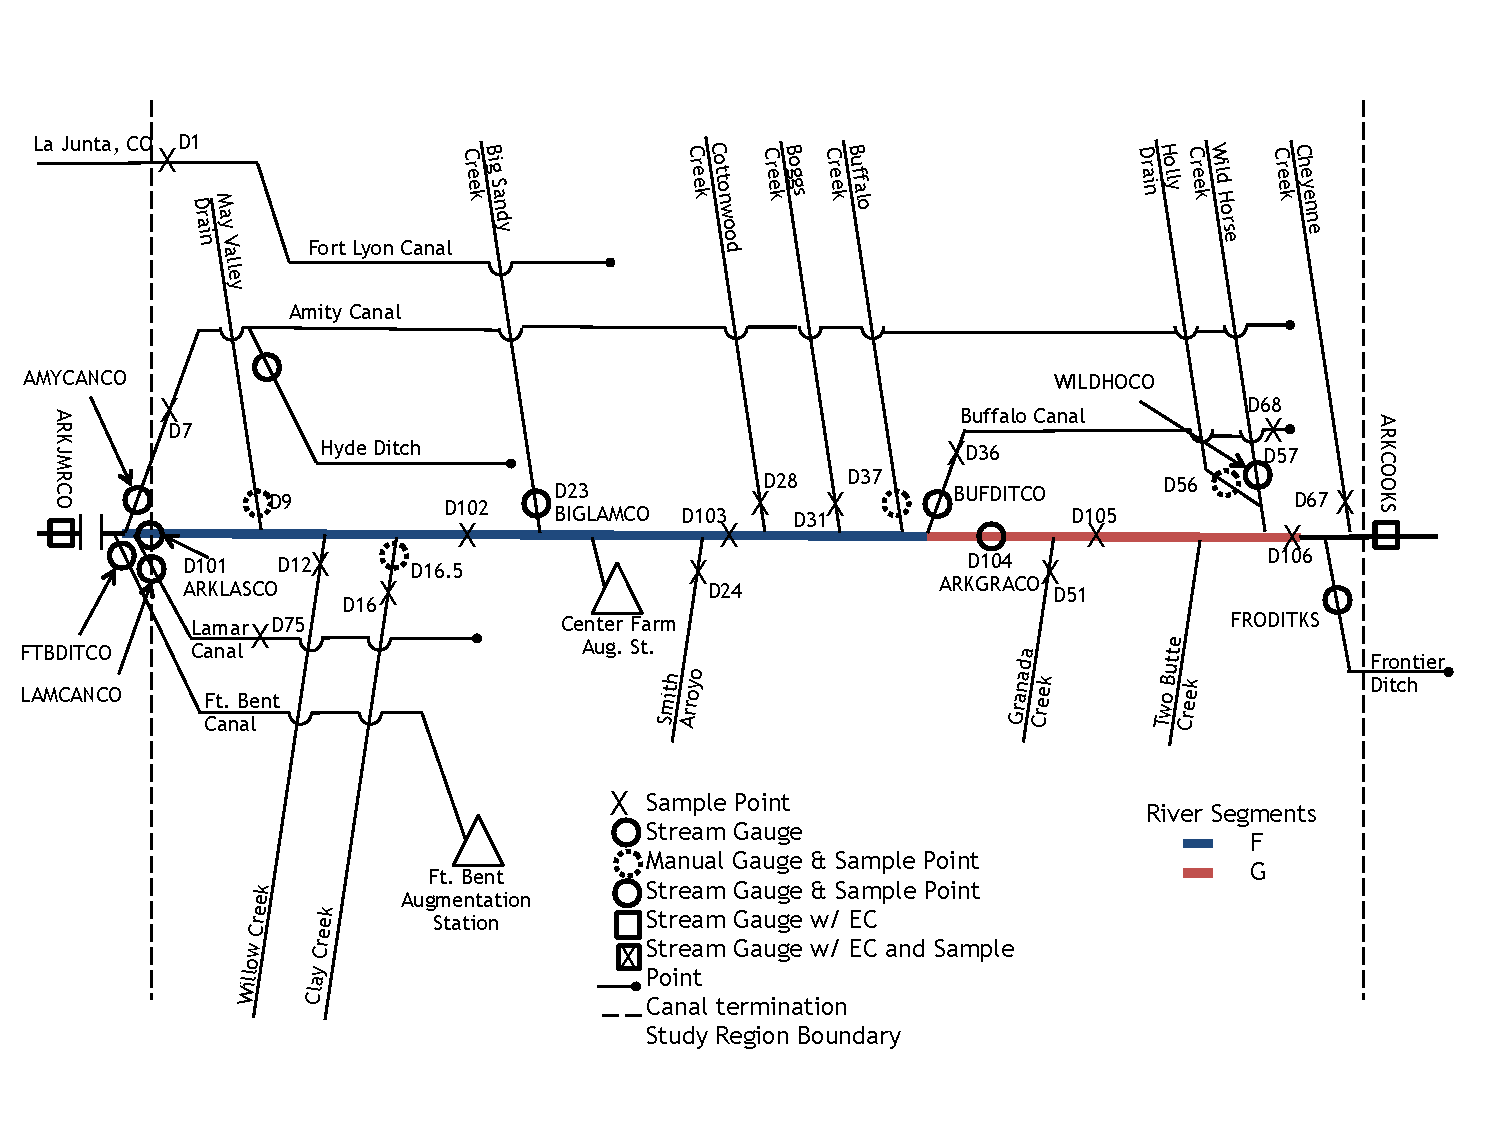
\includegraphics[width=9in]{Figures/LineDiagram/DSRLineDiagram}
			\caption[Downstream Study Reach Flow Diagram.]{Downstream Study Reach Flow Diagram.}
			\label{fig:DSR line map}
	\end{figure}
	\end{landscape}
}

The DSR is separated into Segment F and Segment G as shown in figure \ref{fig:DSR map}. The diversion dam for the Buffalo Ditch irrigation canal is the boundary between the two DSR segments.  Field technicians have observed complete diversion of the Arkansas River at the Buffalo Ditch diversion with small but significant flows reappearing in the Arkansas River channel only a few kilometers downstream.  This leads to the speculation that significant portions of the downstream in-channel flow are from groundwater return flow.

The major tributaries within the DSR are Big Sandy Creek and Wild Horse Creek.  CSU field technicians have observed that the stream gauge on Big Sandy Creek has been affected by beaver dams constructed downstream of the gauge and upstream of the culvert passing under State Highway 196.  The stream gauge on Wild Horse Creek is operated seasonally from April through November.  CSU has made many visual flow observations in these creeks outside of the irrigation season.  The off season flows are either extremely low or the stream is frozen.

Unlike the USR, most of the minor tributaries in the DSR flow most of the year except in drought conditions.  The primary source of water in the minor tributaries is irrigation runoff flowing into the streams through surface and subsurface flow paths.  Most minor tributaries in the DSR do not have definitive entry points to the Arkansas River channel resulting in doubt as to whether these flows reach the Arkansas River as surface water.  It was assumed herein that the minor tributary flows enter the main stem primarily as groundwater.  Minor surface return flows that do reach the Arkansas River are not gauged and most are difficult to access. 

Buffalo Canal is the only functioning canal diversion within the DSR.  There is historical and aerial imagery evidence for another diversion, but the Arkansas River has been routed around the structure and neither the CDWR nor the USGS maintain a flow gauge for the canal serviced by the diversion.

\end{linenumbers}
\clearpage{}